\section{Data}\label{sec:sims}
\subsection{Illustris TNG} \label{sec:tng}
\todo{describe what galaxy properties (SFH, ZH, etc) are available} 

\subsection{SIMBA} \label{sec:tng}
\todo{describe what galaxy properties (SFH, ZH, etc) are available} 

\subsection{Spectral Energy Distributions} \label{sec:sed}
\todo{describe how the SED is generated using the SFH and ZHs} 

\subsection{Forward Modeling SDSS Photometry and Spectra} \label{sec:fm} 


\subsection{SDSS DR7 Central Galaxies} \label{sec:obs} 
We compare the simulations above to central galaxies sample from the \cite{tinker2011} SDSS group catalog. The
\cite{tinker2011} group catalog, first, selects volume-limited sample of galaxies 
at $z \approx 0.04$ with $M_r < -18$ and complete above $M_* > 10^{9.4}
h^{-2}M_\odot$ from the NYU Value-Added Galaxy Catalog~\citep[VAGC;][]{blanton2005} 
of SDSS DR7~\citep{abazajian2009}. The stellar masses are estimated using the
$\mathtt{kcorrect}$ code~\citep{blanton2007a} assuming a~\cite{chabrier2003}
initial mass function.

Central galaxies are then identified using a halo-based group finder that uses
the abundance matching ansatz to iteratively  assign halo masses to groups.
Every group contains one central galaxy, which by definition is the most
massive, and a group can contain $\ge0$ satellites. As with any group finder,
galaxies are misassigned due to projection effects and redshift space
distortions; however, the central galaxy sample has a purity of ${\sim}90\%$
and completeness of ${\sim}95\%$~\citep{tinker2018}. 

In Figure~\ref{fig:smf}, we present the stellar mass function (SMF) of our SDSS
central galaxy sample along with central galaxy SMFs of the SIMBA (orange) and
TNG (blue) simulations. The uncertainties for the SDSS SMF are derived from
jackknife resampling. Although we present the SMFs for reference, we do not use
stellar masses throughout the paper since they are inconsistently defined among
simulations and observations. Instead, we compare between the simulations and
SDSS using luminosity, $M_r$, which we consistently forward model and measure
in the simulations. In these comparisons, we restrict ourselves to galaxies
brighter than $M_r < -20$, where our SDSS central galaxy sample is complete. 

\begin{figure}
\begin{center}
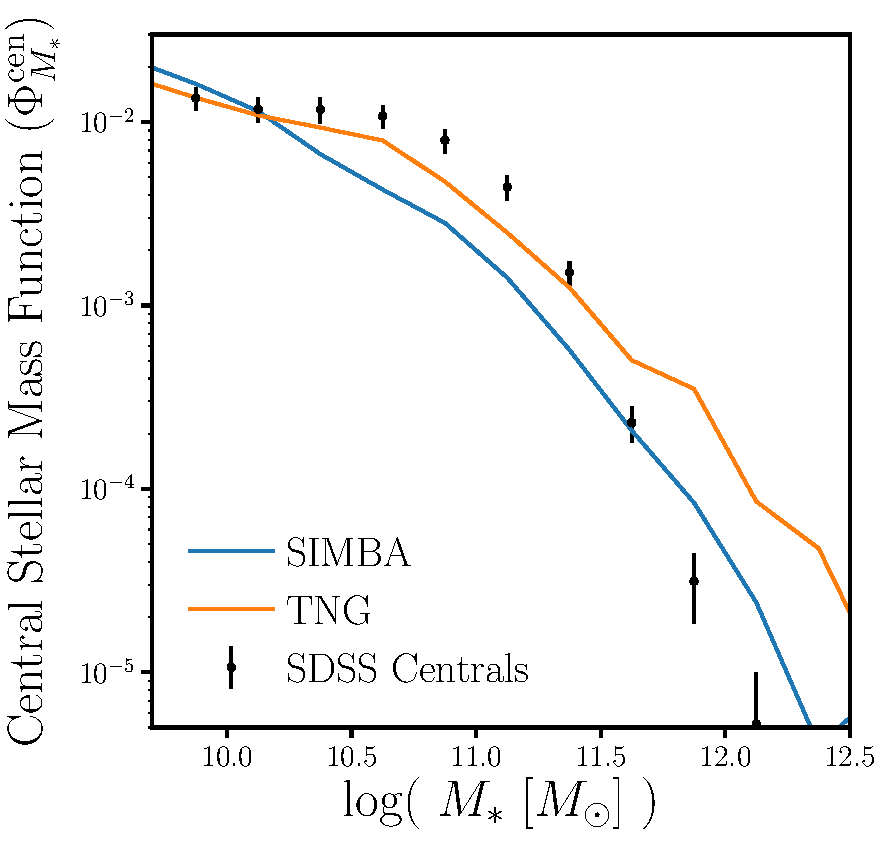
\includegraphics[width=0.5\textwidth]{figs/smfs.pdf} 
    \caption{The stellar mass functions of central galaxies from the SIMBA
    (orange) and TNG (blue) simulations compared to the central SMF of SDSS
    (Section~\ref{sec:obs}). The uncertainties for the SDSS SMF is derived
    using jackknife resampling.}
\label{fig:smf}
\end{center}
\end{figure}

